% This is based on "sig-alternate.tex" V1.9 April 2009
% This file should be compiled with V2.4 of "sig-alternate.cls" April 2009
%
\documentclass{sig-alternate}

\usepackage[english]{babel}
\usepackage{graphicx}
\usepackage{tabularx}
\usepackage{subfigure}
\usepackage{enumitem}
\usepackage{url}
\usepackage{listings}
\usepackage{bookmark}
\usepackage{hyperref} % hyperref for links
%\PassOptionsToPackage{pdfpagelabels=true}{hyperref} % the sig-alternate.tex breaks hyperref, this should fix it again and get rid of the warning


\usepackage{color}
\definecolor{orange}{rgb}{1,0.5,0}
\definecolor{lightgray}{rgb}{.9,.9,.9}
\definecolor{java_keyword}{rgb}{0.37, 0.08, 0.25}
\definecolor{java_string}{rgb}{0.06, 0.10, 0.98}
\definecolor{java_comment}{rgb}{0.12, 0.38, 0.18}
\definecolor{java_doc}{rgb}{0.25,0.35,0.75}

% code listings

\usepackage{listings}
\lstloadlanguages{Java}
\lstset{
	language=Java,
	basicstyle=\scriptsize\ttfamily,
	backgroundcolor=\color{lightgray},
	keywordstyle=\color{java_keyword}\bfseries,
	stringstyle=\color{java_string},
	commentstyle=\color{java_comment},
	morecomment=[s][\color{java_doc}]{/**}{*/},
	tabsize=2,
	showtabs=false,
	extendedchars=true,
	showstringspaces=false,
	showspaces=false,
	breaklines=true,
	numbers=left,
	numberstyle=\tiny,
	numbersep=6pt,
	xleftmargin=3pt,
	xrightmargin=3pt,
	framexleftmargin=3pt,
	framexrightmargin=3pt,
	captionpos=b
}

% Disable single lines at the start of a paragraph (Schusterjungen)

\clubpenalty = 10000

% Disable single lines at the end of a paragraph (Hurenkinder)

\widowpenalty = 10000
\displaywidowpenalty = 10000
 
% allows for colored, easy-to-find todos

\newcommand{\todo}[1]{\textsf{\textbf{\textcolor{orange}{[[#1]]}}}}

% consistent references: use these instead of \label and \ref

\newcommand{\lsec}[1]{\label{sec:#1}}
\newcommand{\lssec}[1]{\label{ssec:#1}}
\newcommand{\lfig}[1]{\label{fig:#1}}
\newcommand{\ltab}[1]{\label{tab:#1}}
\newcommand{\rsec}[1]{Section~\ref{sec:#1}}
\newcommand{\rssec}[1]{Section~\ref{ssec:#1}}
\newcommand{\rfig}[1]{Figure~\ref{fig:#1}}
\newcommand{\rtab}[1]{Table~\ref{tab:#1}}
\newcommand{\rlst}[1]{Listing~\ref{#1}}

% General information

\title{einz\\
\normalsize{Distributed Systems -- Project Proposal}}
\subtitle{subtitle}

% Use the \alignauthor commands to handle the names
% and affiliations for an 'aesthetic maximum' of six authors.

\numberofauthors{6} %  in this sample file, there are a *total*
% of EIGHT authors. SIX appear on the 'first-page' (for formatting
% reasons) and the remaining two appear in the \additionalauthors section.
%
%\author{
% You can go ahead and credit any number of authors here,
% e.g. one 'row of three' or two rows (consisting of one row of three
% and a second row of one, two or three).
%
% The command \alignauthor (no curly braces needed) should
% precede each author name, affiliation/snail-mail address and
% e-mail address. Additionally, tag each line of
% affiliation/address with \affaddr, and tag the
% e-mail address with \email.
%
% 1st. author
%\alignauthor \normalsize{Clemens Bachmann, Josua Cantieni, Fabian Gessler, Christian Knieling, Eric Mink, Silvia Siegrist}\\
%	\affaddr{\normalsize{ETH ID-1 13-932-488, ETH ID-2 15-919-038, ETH ID-3 15-939-341, ETH ID-4 14-923-809, ETH ID-5 15-917-057, ETH ID-6 15-935-893}}\\
%	\email{\normalsize{baclemen@student.ethz.ch, two@student.ethz.ch, fgesser@student.ethz.ch, knielinc@student.ethz.ch, minker@student.ethz.ch, %sisilvia@student.ethz.ch}}
%}
%TODO: überprüefed eui agabe

\author{
\alignauthor
\normalsize{Clemens Bachmann}\\
	\affaddr{\normalsize{13-932-488}}\\
	\email{\normalsize{baclemen@student.ethz.ch}}
%
\alignauthor
\normalsize{Josua Cantieni}\\
	\affaddr{\normalsize{15-919-038}}\\
	\email{\normalsize{josuac@student.ethz.ch}}
%
\alignauthor
\normalsize{Fabian Gessler}\\
	\affaddr{\normalsize{15-939-341}}\\
	\email{\normalsize{fgessler@student.ethz.ch}}
\and
\alignauthor
\normalsize{Christian Knieling}\\
	\affaddr{\normalsize{ 14-923-809}}\\
	\email{\normalsize{knielinc@student.ethz.ch}}
%
\alignauthor
\normalsize{Eric Mink}\\
	\affaddr{\normalsize{15-917-057}}\\
	\email{\normalsize{minker@student.ethz.ch}}
%
\alignauthor
\normalsize{Silvia Siegrist}\\
	\affaddr{\normalsize{15-935-893}}\\
	\email{\normalsize{sisilvia@student.ethz.ch}}
}

\begin{document}

\maketitle

\begin{abstract}
We chose to create an android application which allows to play the game "einz" which is very similar to the popular UNO cardgame. The goal is to be able to play this game with friends wherever you are and with the rules you are used to, as long as you have an android smartphone and access to the same local area network.

For this purpose we will create an android application which is able to take the role of server and client at the same time. The device of one of the players is used as the server for the game which saves the state of the game and is responsible for synchronization. In this way, there is no extra server needed.
\end{abstract}

\section{Introduction}
We build a distributed game similar to the known card game "UNO" by Mattel~\cite{unoshop}. Because you might often find yourself wanting to play a game with friends - e.g. while you are waiting for the next train - but without a set of cards to play it, therefore it would be useful to always carry the cards on you. We make this easy by implementing a similar game on the phone as a native application.

Obvious difficulties awaiting us include the coordination of a team consisting of six people, each with different skillsets and time available.
Also, we intend to create an easily extensible codebase so that we can first build the base game and in a second phase add further rules without much effort. This poses difficulties on its own as we have to learn coding patterns such as using factories to make the program code more modular.

Technical problems will probably be the smooth and clean communication between the clients and the server and implementing concurrency within the server itself. For the networking difficulties like message ordering and making sure the peers actually get the messages, we will rely on TCP using the \verb|Socket| class~\cite{socketdoc}. There remains the problem of noticing if a client loses connection unexpectedly, especially because we might have times where we don't need to send messages at all for multiple seconds for example if it's not a players turn. We have to experiment with that problem and probably add a ping message that checks that the connection is still alive.


\section{System Overview}
We propose a modular approach, building first the baseline functionality of the game, followed by further improvements like additional rules for the game. The baseline functionality of the game is a playable version of UNO where only the most basic cards are featured. Further cards will be implemented as rules, e.g. the rule "We feature a +2 card". The additional rules will be available to the user of the device the server runs on before the game starts, such that we can dynamically change the way the game works. This does not mean that we intend to allow the user to define their own rules - just that they can choose which rules should be applied.

\subsection{Server Client Messaging}
\begin{figure}[!htbp]
\begin{verbatim}
{
  "header":{
    "messagegroup":"registration",
    "messagetype":"Register"
  },
  "body":{
    "username":"roger",
    "role":"player"
  }
}
\end{verbatim}
\caption{Example: Request to register user}
\lfig{regmsg}
\end{figure}

First of all, we implement a simple server-client setup and define the format and the messages that should be provided as an interface between the client and the server.(See our first~\cite{messaging} and second~\cite{messaging2} draft) At the same time, we can start implementing the user interface and writing this proposal.

See~\rfig{regmsg} for an example of how our messages will be structured. We encode all our messages in JSON and split them into a header, which is uniform over all messages, and a body, which is message-specific in content. To parse these messages, we implement factories to make the code modular.

That is, the \verb|ParserFactory| use the \verb|messagegroup| to create a \verb|Parser| object specific to the kind of message. Which \verb|Parser| to choose is decided via a dynamically registered mapping, which means that we can reuse the code on both the server and the client side, and that we have minimal effort if we need to change or add some type of message.

For example, say that we need to add a timestamp to the \verb|Register| message for some reason. Chances are that we also need to update the format of the response to this request, which for this reason has the same \verb|messagegroup|. All of this can be done by changing only the \verb|Parser| for this specific messagegroup.

Once the message is parsed by the \verb|Parser| we use an \verb|ActionFactory| and the \verb|messagetype| to actually turn the specific message into an executable method.

If you're interested in the most current specifications of the messages, see our github page~\cite{github}. There will at some point also be specified how we handle loss of connection, probably using our own implementation of keep-alive packets.

In a second step, once the basic communication between server and client is completed and the exact behaviour of the two parts has been defined, we finish implementing the server-side game logic and start using the previously defined messaging functionality.

We plan that the server does most of the computations and only sends the client its state, containing the players hand, the number of cards other players are holding and the most recently played cards. The client receives also a list of possible actions that he is able to do. For example the server informs the client which cards are playable. The client can now choose an action from the list and send a request to the server afterwards. The server will handle the request and check if it is a valid request. If it is he will inform all clients about the updated state.

Sending the actions to the client allows us later on to add game-modes and rules with ease and grants us high flexibility with using the rules. We only have to change a few files to add new content - ideally just one.

We are also trying to keep the classes themselves very modular to keep updating them - e.g. by adding further rules - just as simple.

\subsection{User Interface}

\begin{figure}[!htbp]
	\centering
    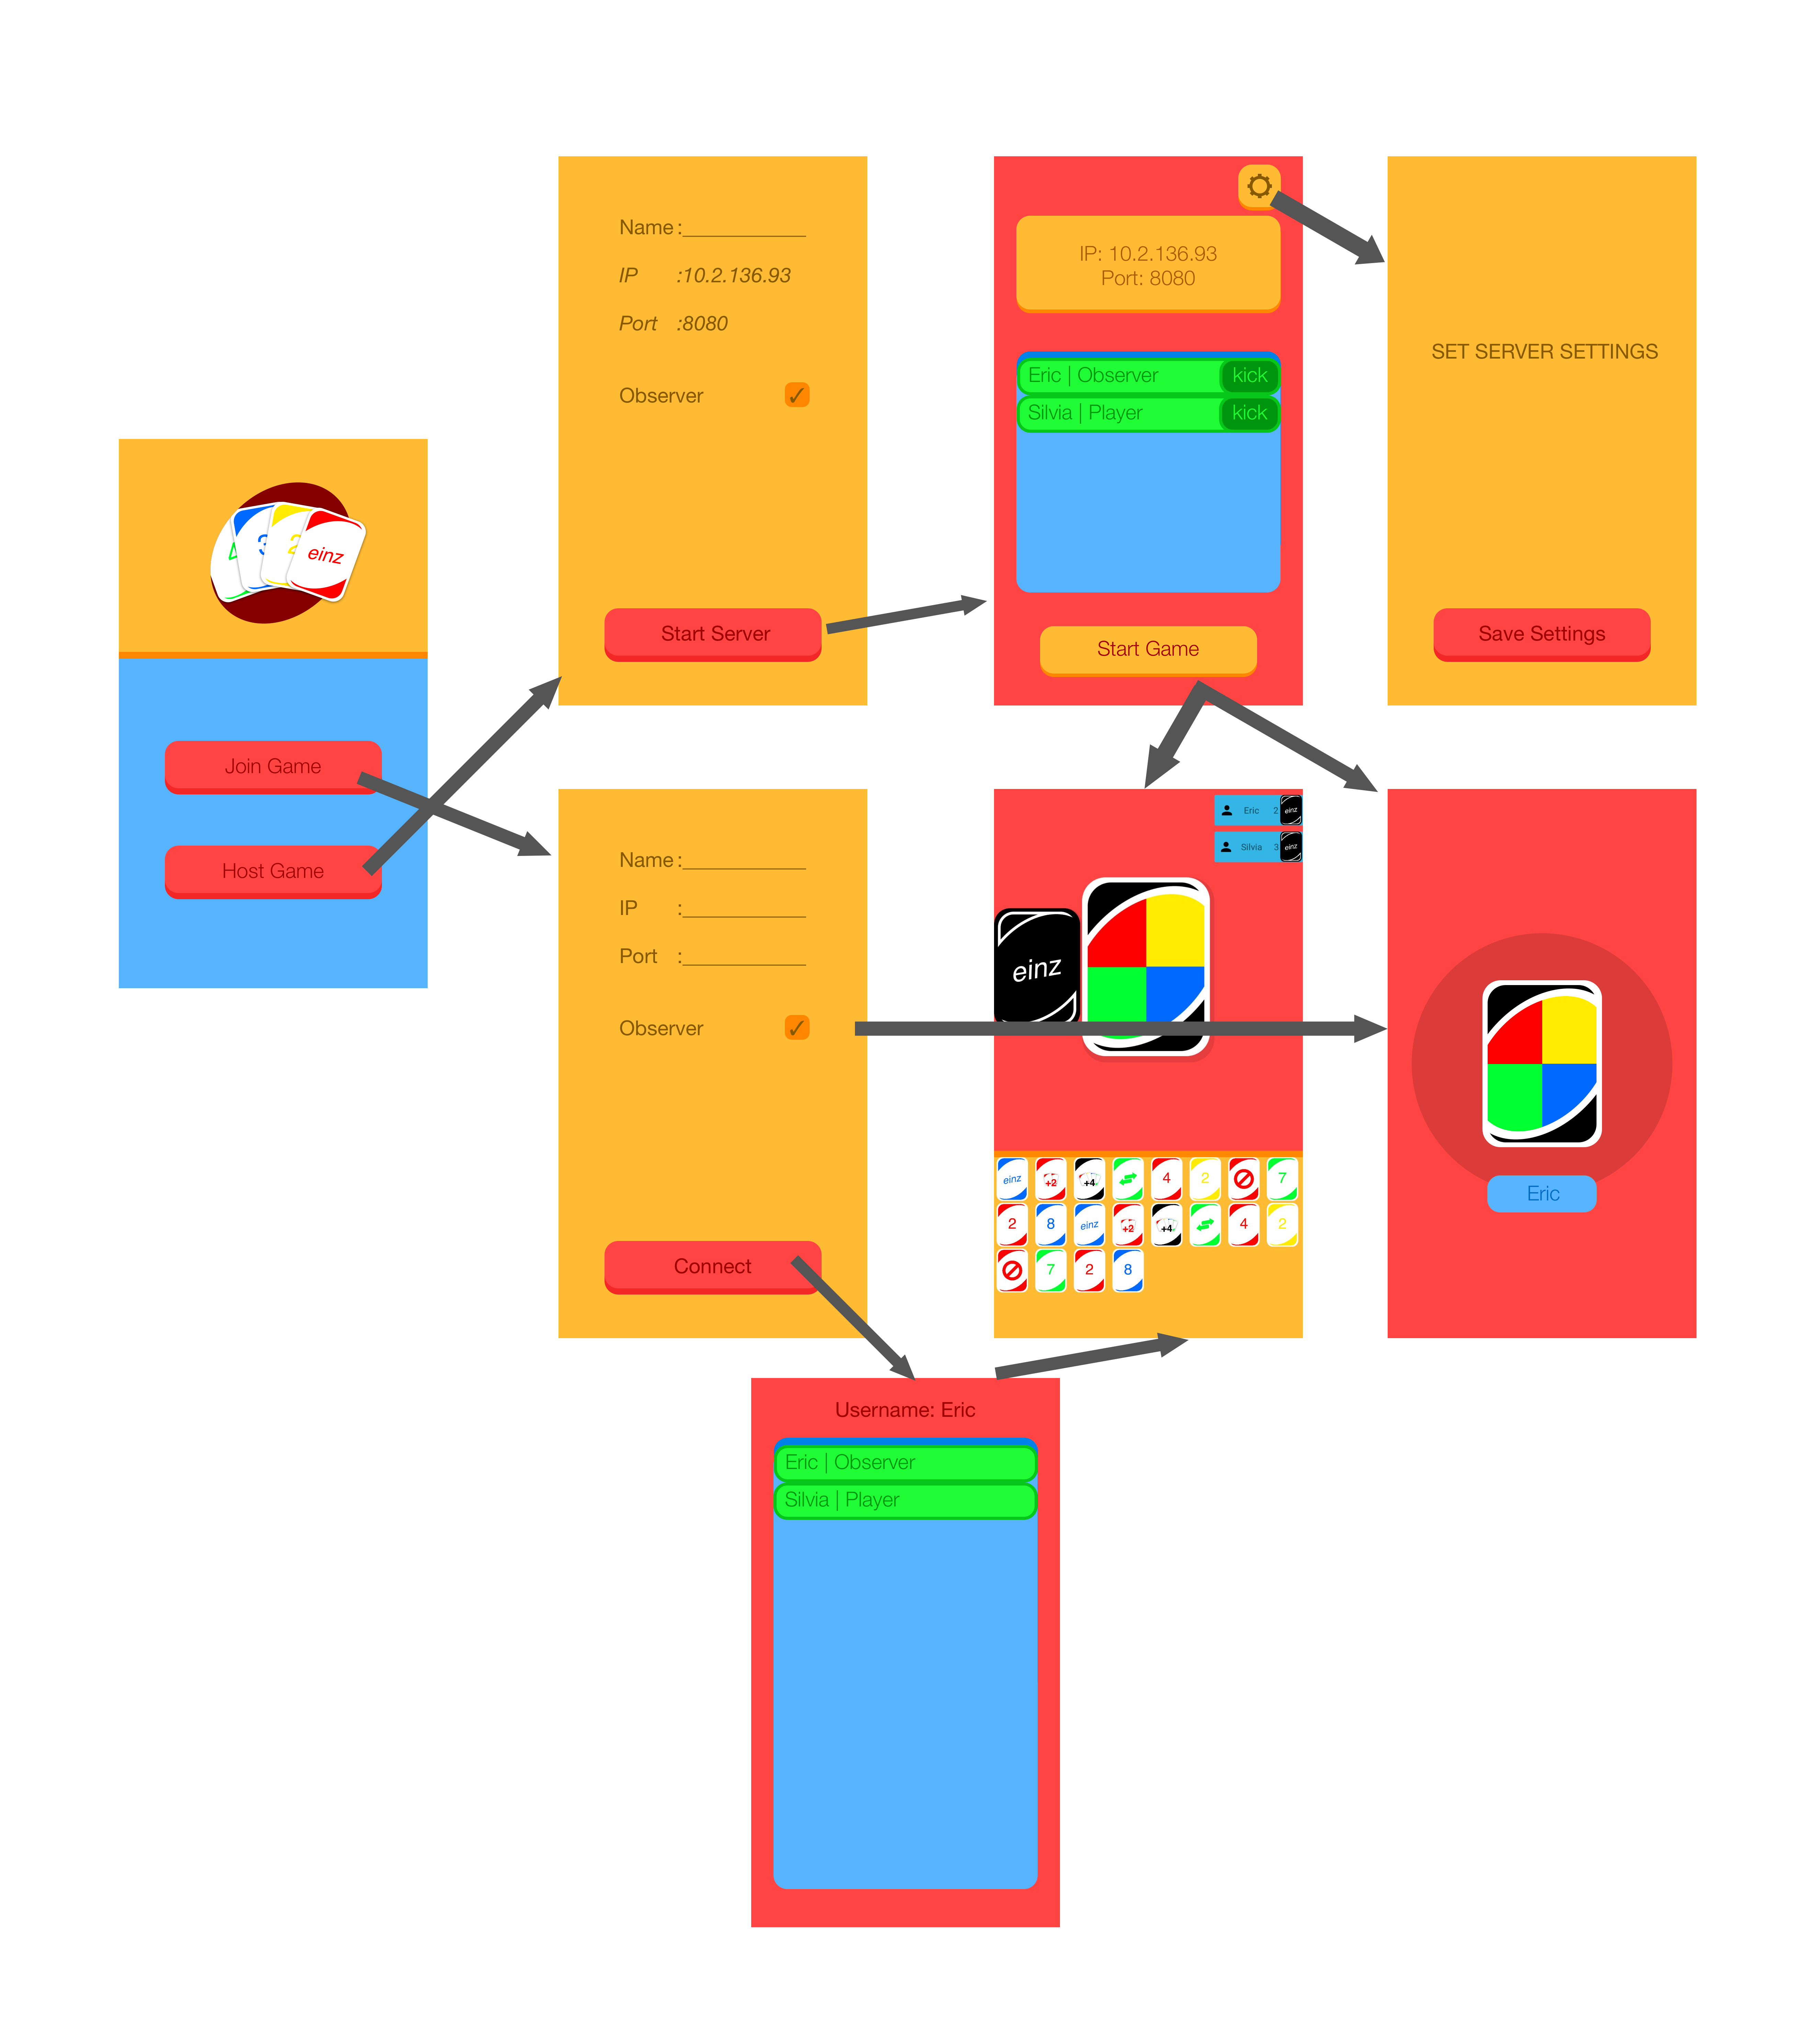
\includegraphics[width=\columnwidth]{Artboard.png}
    \vspace{-5mm} % use negative white space to fix too large gaps
	\caption{User Interface}
	\lfig{artboard}
\end{figure}

The user-interface for the standard scenario from starting the app to start playing looks like the following: The first screen (1) is for the player to choose, whether he wants to start a new game or join an already existing game. If he decides to start a new one, he will start the server in a thread in the background. He will be prompted to enter his username and decide whether he wants to play or observe/spectate the game. If he presses the "Start Server" Button in (2) after filling out the missing information, he will connect himself as an administrator to the previously started server running in the background of his device. After that he will be forwarded to an activity (3), with the necessary information for others to connect and a list of already connected players/observers. He can kick them if he decides to do so. By pressing the settings button he will be taken to (4) and there he can specify the rules for the game.

A client that joins a game will go through a similar process. He has to start by filling out his name, the host IP and port and whether he wants to act as a player or a spectator (5). Once the player connects to the server he will see a list of other players/observers, but not be able to kick them or change any settings, as this is left for the host/admin (8). 

When the host starts the game, everyone will see the activity in which the game itself will take place - either a standard view with his hand, the topmost card, all connected players and the amount of cards in each hand (6) or the view of the spectator (7). Players will be able to play any card that is declared as playable by the server or draw cards from the heap. A player arbitrarily leaving the game by pressing the back button is also an action that we take into consideration.

Spectators will see the public game-state, but not any players hand cards. Also they will not be able to interact with the game in any way. The use-case for this option is that you could place a - possibly larger - android device (tabled, phablet) in the middle of a table to get the "classic cardgame feel" with a physical representation of the stack of discarded cards while still playing on mobile devices. 

\subsection{Dynamic Rules}
Since every group plays UNO with different rules we want to provide them with the possibility to play by the rules they are used to. We will feature a setting-screen for the admin where he can specify the rules for the next game. These will mostly be checkboxes or multiple-choice dropdown menus. This means that we will not feature user-designed rules. However, we intend to make use of the efforts we put into the extensibility of our codebase by adding the ideas we had during our first meeting~\cite{firstprotocol} if we have enough time to do so.

\subsection{Organizing}
Working in a larger team and managing it is new to us. We try to help ourselves by using git with github~\cite{github} and trello~\cite{trello} to manage the tasks. We have also appointed a Team Lead whose task it is to distribute the work so that everybody can contribute meaningfully to the Project yet also learn something while doing so. 

\subsection{Additional Possible Goals}
Once the game is in a working state with a few rules such as an additional card like the one where the player can choose a color or the well-known "+2" card from UNO, we will decide whether we need to focus on bug-fixing, cleaning up code, implementing a lookup-server (LUS) for NAT-traversal~(See~\rfig{nat}) or adding more rule options. 

\begin{figure}[!htbp]
	\centering
    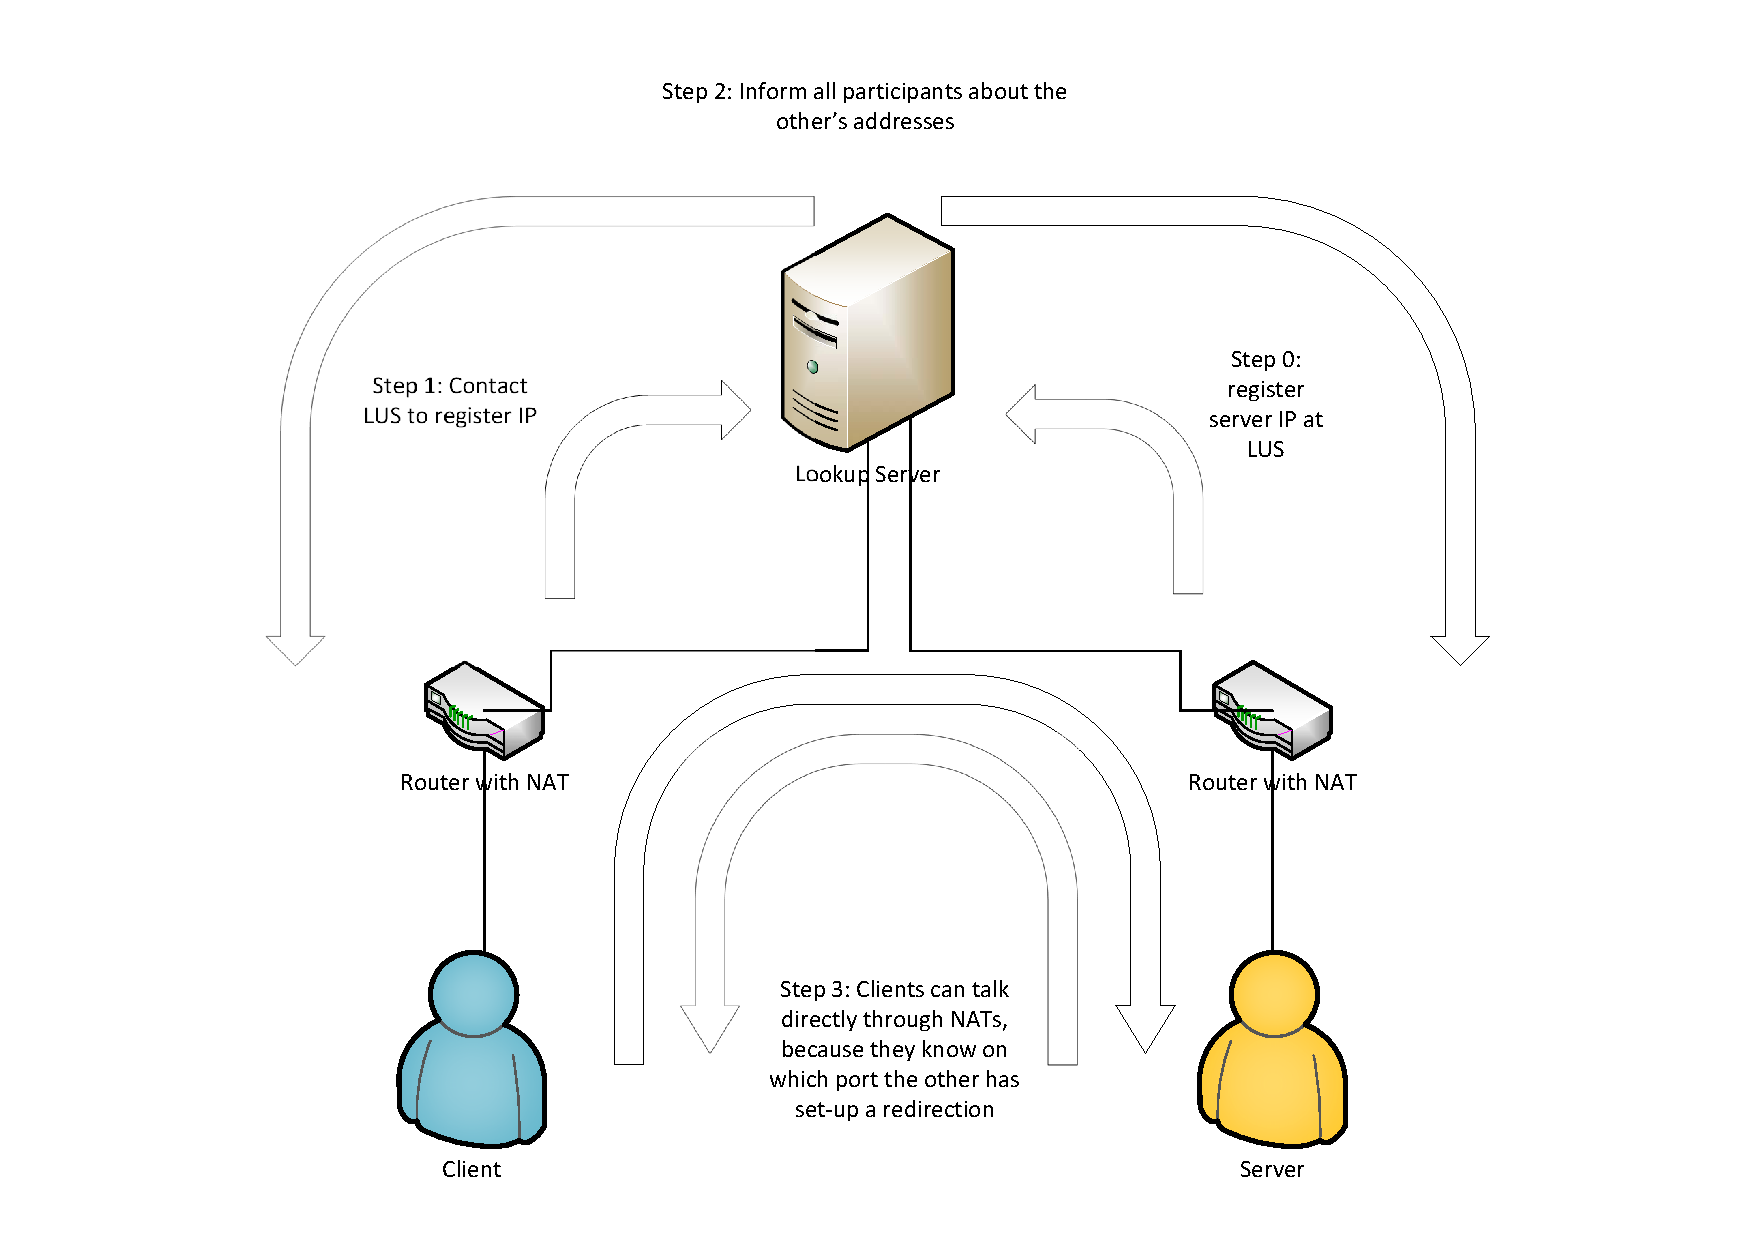
\includegraphics[width=\columnwidth]{NATholepunching.pdf}
    \vspace{-5mm} % use negative white space to fix too large gaps
	\caption{NAT-traversal}
	\lfig{nat}
\end{figure}

If we find enough time after adding enough rules to make the game interesting - we probably will not - and decide to do NAT traversal, we would set up a Lookup-server that is reachable for all clients and thus allow the routers to setup forwarding on ports that we know. The LUS can then inform every client about the servers's IP address and ports, through which they can communicate the same way as we implemented in the first phase (And vice-versa. See~\rfig{nat}). The gameserver on one phone will have the option to choose whether to use the LUS or only accept players from within the same LAN.

Adding a LUS might impose additional difficulties because some mobile carriers might use symmetric NATs.~\cite{natwiki}If these difficulties arise, we will probably resort to only implementing NAT-traversal for the other (easier) types of NATs.

\section{Requirements}
The app will run on Android devices that run at least Android 5.0, which correspond to the API-level 21. We use the local wireless connection to communicate between the devices. Thus we need the permissions \verb|INTERNET| and \verb|ACCESS_WIFI_STATE|

Since this is a multi-player game we also need more than one device that are able to communicate through the local WiFi with each other for the game to run.

\section{Work Packages}
There work will be broken down into the following subtasks:

\begin{itemize}
	
        \item {\bf WP1}: Define Client-Server Communication\\
        We define the protocol that the client and the server use to communicate. Once we agreed on a message exchange protocol, the development of the server and the client can be done separately.
        
        \item {\bf WP2}: Design and implement Game Model\\
        Implement the data-structure and objects used by both client and server. This means classes like gamestate, card and rules
        
        \item {\bf WP3}: Server Game Logic\\
        Implement the game logic without thinking about the networking part or multi-threading
        
        \item {\bf WP4}: Dynamic Message Parser\\
		Implement a reusable parsing system that maps the incoming messages to executable methods as described in the System Overview.
           
        \item {\bf WP5}: Client Communication Backend\\
		Implement message parsing on the client side
		
		\item {\bf WP6}: Server Backend\\
		Implement message parsing in the server side
		
		\item {\bf WP7}: Implement Client Server Protocol\\
		Register parsers and actions for every type of message specified. The server could implement this in multiple threads and has thus to call the actions in a safe way.
		
		\item {\bf WP8}: Connect Server-logic to Messaging\\
		Messages should be parsed and the corresponding action should be executed. The logic calls back to the messaging part to inform the clients about updates in the game-state.
		\item {\bf WP9}: Application UI\\
		Make a UI like previously described for all the different Activities. Add resourced for them all to have the same style.
		
		\item {\bf WP10}: Polish the Game and Bugfixes\\
		Optimize the user experiences and fix all those nasty bugs.
		
		\item {\bf WP11}: Implement Additional Rules:\\
		Rules to make each game individual.
		
		\item {\bf Optinal WP}: If there is time implement additional goals\\
        Only if we really have the time. We can implement the ideas we had in section "Additional Possible Goals"
        
\end{itemize}

\section{Milestones}

\subsection{Milestone 1: Specification}
Specify the interfaces and get ready for implementation
\begin{itemize}
	\item WP1 - Eric, Fabian, Josua
	\item WP2 - Josua
\end{itemize}
Due: 19.11.2017

\subsection{Milestone 2: Fundamental}
Laying the foundation for the client-server messaging on both the client and the server
\begin{itemize}
	\item WP4 - Eric
	\item WP5 - Christian, Clemens
	\item WP6 - Eric, Silvia
\end{itemize}
Due: 26.11.2017
	
\subsection{Milestone 3: Messaging}
Implement and test the previous specified messaging protocol
\begin{itemize}
	\item WP7 - Eric, Silvia
\end{itemize}
Due: 30.11.2017

\subsection{Milestone 4: Base Game}
Getting the game to work in a basic fashion
\begin{itemize}
	\item WP3 - Fabian
	\item WP8 - Eric , Fabian
	\item WP9 - Christian
\end{itemize}
Due: 7.12.2017

\subsection{Milestone 5: Final Game}
Implement additional rules and test and polish the game.
\begin{itemize}
	\item WP10 - Everyone
	\item WP11 - Everyone
\end{itemize}
Due: 17.12.2017

Before we start to code, we first write a specification for the interfaces to prevent a big mess. For the implementation we see two areas where we assign our team members to: the server and the client. Also someone is something like the tech-lead and keeps an overview about the entire process.

For the server we assign Eric and Fabian and Silva

For the client we assign Christian and Clemens.

Josua tries to keep an eye over the whole project.



% The following two commands are all you need in the
% initial runs of your .tex file to
% produce the bibliography for the citations in your paper.
\bibliographystyle{abbrv}
\bibliography{report}  % sigproc.bib is the name of the Bibliography in this case
% You must have a proper ".bib" file

%\balancecolumns % GM June 2007

\end{document}
